
\blankAteven
\pagestyle{empty}
\begingroup
\rmfamily
\fontsize{7}{8}\selectfont

\color{black}


{%
  \IfFileExists{img/HEDRA_EDICOES.pdf}{%
    \vspace*{0mm}%
    \begin{enumerate}
      \setlength{\topsep}{0pt}\setlength{\partopsep}{0pt}\setlength{\itemsep}{0pt}\setlength{\parsep}{0pt}
      \item[] \noindent\hspace*{-1em}
\includegraphics[width=.42\textwidth,keepaspectratio]{img/HEDRA_EDICOES.pdf}\par
    \end{enumerate}
  }{\large\textsc{hedra edições}}%
}



% Hide enumerate labels but keep default indentation
\makeatletter
\renewcommand{\labelenumi}{}
\renewcommand{\labelenumii}{}
\renewcommand{\labelenumiii}{}
\makeatother
% Slightly reduce left indentation of enumerate items (local to this group)
%\addtolength{\leftmargini}{-1.8em}
%\addtolength{\leftmarginii}{-1.8em}
%\addtolength{\leftmarginiii}{-1.8em}

\begin{enumerate}
\setlength{\topsep}{2pt}
\setlength{\partopsep}{0pt}
\setlength\parskip{4.2pt}
\setlength\itemsep{-1.4mm}
\item \textit{A arte da guerra}, Maquiavel
\item \textit{A cruzada das crianças\,/\,Vidas imaginárias}, Marcel Schwob
\item \textit{A filosofia na era trágica dos gregos}, Friedrich Nietzsche
\item \textit{A fábrica de robôs}, Karel Tchápek 
\item \textit{A história trágica do Doutor Fausto}, Christopher Marlowe
\item \textit{A metamorfose}, Franz Kafka
\item \textit{A monadologia e outros textos}, Gottfried Leibniz
\item \textit{A morte de Ivan Ilitch}, Lev Tolstói 
\item \textit{A velha Izerguil e outros contos}, Maksim Górki
\item \textit{A vida é sonho}, Calderón de la Barca
\item \textit{A volta do parafuso}, Henry James
\item \textit{A voz dos botequins e outros poemas}, Paul Verlaine 
\item \textit{A vênus das peles}, Leopold von Sacher{}-Masoch
\item \textit{A última folha e outros contos}, O.\,Henry
\item \textit{Americanismo e fordismo}, Antonio Gramsci
\item \textit{Apologia de Galileu}, Tommaso Campanella 
\item \textit{Arcana C\oe lestia} e \textit{Apocalipsis revelata}, Emanuel Swedenborg
\item \textit{Autobiografia de uma pulga}, [Stanislas de Rhodes]
\item \textit{Balada dos enforcados e outros poemas}, François Villon
\item \textit{Carmilla, a vampira de Karnstein}, Sheridan Le Fanu
\item \textit{Carta sobre a tolerância}, John Locke
\item \textit{Contos clássicos de vampiro}, L.\,Byron, B.\,Stoker \& outros
\item \textit{Contos de amor, de loucura e de morte}, Horacio Quiroga
\item \textit{Contos indianos}, Stéphane Mallarmé
\item \textit{Cultura estética e liberdade}, Friedrich von Schiller
\item \textit{Dao De Jing}, Lao Zi
\item \textit{Discursos ímpios}, Marquês de Sade
\item \textit{Dissertação sobre as paixões}, David Hume
\item \textit{Diário de um escritor} (1873), Fiódor Dostoiévski
\item \textit{Diário parisiense e outros escritos}, Walter Benjamin
\item \textit{Diários de Adão e Eva}, Mark Twain
\item \textit{Don Juan}, Molière
\item \textit{Dos novos sistemas na arte}, Kazimir Maliévitch
\item \textit{Educação e sociologia}, Émile Durkheim
\item \textit{Elogio da loucura}, Erasmo de Rotterdam
\item \textit{Émile e Sophie ou os solitários}, Jean-Jacques Rousseau 
\item \textit{Emília Galotti}, Gotthold Ephraim Lessing
\item \textit{Ernestine ou o nascimento do amor}, Stendhal
\item \textit{Escritos sobre arte}, Charles Baudelaire
\item \textit{Escritos sobre literatura}, Sigmund Freud
\item \textit{Eu acuso!}, Zola\,/\,\textit{O processo do capitão Dreyfus}, Rui Barbosa
\item \textit{Explosão: romance da etnologia}, Hubert Fichte
\item \textit{Feitiço de amor e outros contos}, Ludwig Tieck
\item \textit{Flossie, a Vênus de quinze anos}, [Swinburne]
\item \textit{Fábula de Polifemo e Galateia e outros poemas}, Góngora
\item \textit{Fé e saber}, Georg W.\,F.\,Hegel
\item \textit{Gente de Hemsö}, August Strindberg 
\item \textit{Hawthorne e seus musgos}, Herman Melville
\item \textit{Imitação de Cristo}, Tomás de Kempis
\item \textit{Incidentes da vida de uma escrava}, Harriet Jacobs
\item \textit{Inferno}, August Strindberg
\item \textit{Investigação sobre o entendimento humano}, David Hume
\item \textit{Jazz rural}, Mário de Andrade
\item \textit{Jerusalém}, William Blake
\item \textit{Joana d'Arc}, Jules Michelet
\item \textit{Ludwig Feuerbach e o fim da filosofia clássica alemã}, Friedrich Engels
\item \textit{Manifesto comunista}, Karl Marx e Friedrich Engels
\item \textit{Memórias do subsolo}, Fiódor Dostoiévski
\item \textit{Micromegas e outros contos}, Voltaire
\item \textit{Narrativa de William W.\,Brown, escravo fugitivo}, William Wells Brown
\item \textit{Nascidos na escravidão: depoimentos norte-americanos}, \textsc{wpa}
\item \textit{No coração das trevas}, Joseph Conrad
\item \textit{Noites egípcias e outros contos}, Aleksandr Púchkin
\item \textit{O casamento do Céu e do Inferno}, William Blake
\item \textit{O cego e outros contos}, \textsc{d.\,h}.\,Lawrence
\item \textit{O chamado de Cthulhu}, \textsc{h.\,p.}\,Lovecraft
\item \textit{O contador de histórias e outros textos}, Walter Benjamin
\item \textit{O corno de si próprio e outros contos}, Marquês de Sade
\item \textit{O destino do erudito}, Johann Fichte
\item \textit{O estranho caso do dr.\,Jekyll e Mr. Hyde}, Robert Louis Stevenson
\item \textit{O fim do ciúme e outros contos}, Marcel Proust
\item \textit{O ladrão honesto e outros contos}, Fiódor Dostoiévski
\item \textit{O livro de Monelle}, Marcel Schwob
\item \textit{O mundo ou tratado da luz}, René Descartes
\item \textit{O novo Epicuro: as delícias do sexo}, Edward Sellon
\item \textit{O pequeno Zacarias, chamado Cinábrio}, \textsc{e.\,t.\,a.},\,Hoffmann
\item \textit{O primeiro Hamlet}, William Shakespeare
\item \textit{O príncipe}, Maquiavel
\item \textit{O que eu vi, o que nós veremos}, Santos-Dumont
\item \textit{O retrato de Dorian Gray}, Oscar Wilde
\item \textit{O sobrinho de Rameau}, Diderot
\item \textit{Ode ao Vento Oeste e outros poemas}, \textsc{p.\,b.},\,Shelley
\item \textit{Ode sobre a melancolia e outros poemas}, John Keats
\item \textit{Oliver Twist}, Charles Dickens
\item \textit{Os sofrimentos do jovem Werther}, Goethe
\item \textit{Para serem lidas à noite}, Ion Minulescu
\item \textit{Pensamento político de Maquiavel}, Johann Fichte
\item \textit{Pequeno-burgueses}, Maksim Górki
\item \textit{Pequenos poemas em prosa}, Charles Baudelaire
\item \textit{Perversão: a forma erótica do ódio}, Robert Stoller
\item \textit{Poemas}, Lord Byron
\item \textit{Poesia basca: das origens à Guerra Civil} 
\item \textit{Poesia catalã: das origens à Guerra Civil} 
\item \textit{Poesia espanhola: das origens à Guerra Civil} 
\item \textit{Poesia galega: das origens à Guerra Civil} 
\item \textit{Pr\ae terita}, John Ruskin
\item \textit{Rashômon e outros contos}, Ryūnosuke Akutagawa
\item \textit{Robinson Crusoé}, Daniel Defoe
\item \textit{Romanceiro cigano}, Federico García Lorca
\item \textit{Sagas}, August Strindberg
\item \textit{Sobre a amizade e outros diálogos}, Jorge Luis Borges e Osvaldo Ferrari
\item \textit{Sobre a filosofia e outros diálogos}, Jorge Luis Borges e Osvaldo Ferrari
\item \textit{Sobre a filosofia e seu método (Parerga e paralipomena)}, Arthur Schopenhauer 
\item \textit{Sobre a liberdade}, Stuart Mill
\item \textit{Sobre a utilidade e a desvantagem da histório para a vida}, Friedrich Nietzsche
\item \textit{Sobre a ética (Parerga e paralipomena)}, Arthur Schopenhauer 
\item \textit{Sobre os sonhos e outros diálogos}, Jorge Luis Borges e Osvaldo Ferrari
\item \textit{Sobre verdade e mentira}, Friedrich Nietzsche
\item \textit{Sonetos}, William Shakespeare
\item \textit{Sátiras, fábulas, aforismos e profecias}, Leonardo da Vinci
\item \textit{Teleny, ou o reverso da medalha}, Oscar Wilde
\item \textit{Triunfos}, Petrarca
\item \textit{Um anarquista e outros contos}, Joseph Conrad
\item \textit{Viagem aos Estados Unidos}, Alexis de Tocqueville
\item \textit{Viagem em volta do meu quarto}, Xavier de Maistre 
\item \textit{Viagem sentimental}, Laurence Sterne
\end{enumerate}



\IfFileExists{img/PAIDEIA.pdf}{%
  \vspace*{0mm}%
  \begin{enumerate}
    \setlength{\topsep}{0pt}\setlength{\partopsep}{0pt}\setlength{\itemsep}{0pt}\setlength{\parsep}{0pt}
    \item[] \noindent\hspace*{-1em}
\includegraphics[width=.42\textwidth,keepaspectratio]{img/PAIDEIA.pdf}\par
  \end{enumerate}
}{\large\textsc{paideia}}



\begin{enumerate}
\setlength{\topsep}{2pt}
\setlength{\partopsep}{0pt}
\setlength\parskip{4.2pt}
\setlength\itemsep{-1.4mm}
\item \textit{A conjuração de Catilina}, Salústio
\item \textit{As bacantes}, Eurípides
\item \textit{Cântico dos cânticos}, [Salomão]
\item \textit{Édipo Rei}, Sófocles
\item \textit{Fedro}, Platão
\item \textit{Hino a Afrodite e outros poemas}, Safo de Lesbos 
\item \textit{Lira grega}, Giuliana Ragusa (org.)
\item \textit{Lisístrata}, Aristófanes
\item \textit{Metamorfoses}, Ovídio
\item \textit{Primeiro livro dos Amores}, Ovídio
\item \textit{Sobre o riso e a loucura}, [Hipócrates]
\item \textit{Teogonia}, Hesíodo
\item \textit{Trabalhos e dias}, Hesíodo
\end{enumerate}



\IfFileExists{img/METABIBLIOTECA.pdf}{%
  \vspace*{0mm}%
  \begin{enumerate}
    \setlength{\topsep}{0pt}\setlength{\partopsep}{0pt}\setlength{\itemsep}{0pt}\setlength{\parsep}{0pt}
    \item[] \noindent\hspace*{-1em}
\includegraphics[width=.42\textwidth,keepaspectratio]{img/METABIBLIOTECA.pdf}\par
  \end{enumerate}
}{\large\textsc{metabiblioteca}}



\begin{enumerate}
\setlength{\topsep}{2pt}
\setlength{\partopsep}{0pt}
\setlength\parskip{4.2pt}
\setlength\itemsep{-1.4mm}
\item \textit{A carteira de meu tio}, Joaquim Manuel de Macedo
\item \textit{A cidade e as serras}, Eça de Queirós
\item \textit{A escrava}, Maria Firmina dos Reis
\item \textit{A família Medeiros}, Júlia Lopes de Almeida 
\item \textit{A pele do lobo e outras peças}, Artur Azevedo
\item \textit{Auto da barca do inferno}, Gil Vicente
\item \textit{Bom crioulo}, Adolfo Caminha
\item \textit{Cartas a favor da escravidão}, José de Alencar
\item \textit{Contos e novelas}, Júlia Lopes de Almeida
\item \textit{Crime}, Luiz Gama
\item \textit{Democracia}, Luiz Gama
\item \textit{Direito}, Luiz Gama
\item \textit{Elixir do pajé: poemas de humor, sátira e escatologia}, Bernardo Guimarães
\item \textit{Eu}, Augusto dos Anjos
\item \textit{Farsa de Inês Pereira}, Gil Vicente
\item \textit{Helianto}, Orides Fontela
\item \textit{História da província Santa Cruz}, Gandavo
\item \textit{Índice das coisas mais notáveis}, Antônio Vieira
\item \textit{Iracema}, José de Alencar
\item \textit{Liberdade}, Luiz Gama
\item \textit{Mensagem}, Fernando Pessoa
\item \textit{Meridiano 55}, Flávio de Carvalho
\item \textit{O Ateneu}, Raul Pompeia
\item \textit{O cortiço}, Aluísio Azevedo
\item \textit{O desertor}, Silva Alvarenga
\item \textit{Oração aos moços}, Rui Barbosa
\item \textit{Pai contra mãe: as origens perdidas de Luiz Gama}, Bruno Rodrigues de Lima
\item \textit{Pai contra mãe e outros contos}, Machado de Assis
\item \textit{Poemas completos de Alberto Caeiro}, Fernando Pessoa
\item \textit{Teatro de êxtase}, Fernando Pessoa
\item \textit{Transposição}, Orides Fontela
\item \textit{Tratado descritivo do Brasil em 1587}, Gabriel Soares de Sousa
\item \textit{Tratados da terra e gente do Brasil}, Fernão Cardim 
\item \textit{Utopia Brasil}, Darcy Ribeiro
\end{enumerate}



\IfFileExists{img/AYLLON.pdf}{%
  \vspace*{0mm}%
  \begin{enumerate}
    \setlength{\topsep}{0pt}\setlength{\partopsep}{0pt}\setlength{\itemsep}{0pt}\setlength{\parsep}{0pt}
    \item[] \noindent\hspace*{-1em}
\includegraphics[width=.42\textwidth,keepaspectratio]{img/AYLLON.pdf}\par
  \end{enumerate}
}{\large\textsc{ayllon}}



\begin{enumerate}
\setlength{\topsep}{2pt}
\setlength{\partopsep}{0pt}
\setlength\parskip{4.2pt}
\setlength\itemsep{-1.4mm}
\item \textit{A toca iluminada}, Max Blecher
\item \textit{Acontecimentos na irrealidade imediata}, Max Blecher
\item \textit{Cabalat shabat: poemas rituais}, Fabiana Gampel Grinberg
\item \textit{Em busca de meus irmãos na América}, Chaim Novodvorsky
\item \textit{Fragmentos de um diário encontrado}, Mihail Sebastian
\item \textit{Israel e Palestina}, Gershon Baskin
\item \textit{Mulheres}, Mihail Sebastian
\item \textit{O Rabi de Bacherach}, Heinrich Heine
\item \textit{Vilna: cidade dos outros}, Laimonas Briedis
\end{enumerate}



\IfFileExists{img/QUE_HORAS_SAO.pdf}{%
  \vspace*{0mm}%
  \begin{enumerate}
    \setlength{\topsep}{0pt}\setlength{\partopsep}{0pt}\setlength{\itemsep}{0pt}\setlength{\parsep}{0pt}
    \item[] \noindent\hspace*{-1em}
\includegraphics[width=.42\textwidth,keepaspectratio]{img/QUE_HORAS_SAO.pdf}\par
  \end{enumerate}
}{\large\textsc{que horas são?}}



\begin{enumerate}
\setlength{\topsep}{2pt}
\setlength{\partopsep}{0pt}
\setlength\parskip{4.2pt}
\setlength\itemsep{-1.4mm}
\item \textit{8/1: A rebelião dos manés}, Pedro Fiori Arantes, Fernando Frias e Maria Luiza Meneses
\item \textit{A linguagem fascista}, Carlos Piovezani \& Emilio Gentile
\item \textit{A sociedade de controle}, J.\,Souza; R.\,Avelino; S.\,Amadeu (org.)
\item \textit{As Big Techs e a guerra total: o complexo militar-industrial-dataficado}, Sérgio A. da Silveira
\item \textit{Ativismo digital hoje}, R.\,Segurado; C.\,Penteado; S.\,Amadeu (org.)
\item \textit{Crédito à morte}, Anselm Jappe
\item \textit{Descobrindo o Islã no Brasil}, Karla Lima
\item \textit{Desinformação e democracia}, Rosemary Segurado
\item \textit{Dilma Rousseff e o ódio político}, Tales Ab'Sáber
\item \textit{Labirintos do fascismo} (v.\,\textsc{i}), João Bernardo
\item \textit{Labirintos do fascismo} (v.\,\textsc{ii}), João Bernardo
\item \textit{Labirintos do fascismo} (v.\,\textsc{iii}), João Bernardo
\item \textit{Labirintos do fascismo} (v.\,\textsc{iv}), João Bernardo
\item \textit{Labirintos do fascismo} (v.\,\textsc{v}), João Bernardo
\item \textit{Labirintos do fascismo} (v.\,\textsc{vi}), João Bernardo
\item \textit{Lugar de negro, lugar de branco?}, Douglas Rodrigues Barros
\item \textit{Lulismo, carisma pop e cultura anticrítica}, Tales Ab'Sáber
\item \textit{Machismo, racismo, capitalismo identitário}, Pablo Polese
\item \textit{Michel Temer e o fascismo comum}, Tales Ab'Sáber
\item \textit{O quarto poder: uma outra história}, Paulo Henrique Amorim
\item \textit{Universidade, cidade e cidadania}, Franklin Leopoldo e Silva
\end{enumerate}



\IfFileExists{img/MUNDO_INDIGENA.pdf}{%
  \vspace*{0mm}%
  \begin{enumerate}
    \setlength{\topsep}{0pt}\setlength{\partopsep}{0pt}\setlength{\itemsep}{0pt}\setlength{\parsep}{0pt}
    \item[] \noindent\hspace*{-1em}
\includegraphics[width=.42\textwidth,keepaspectratio]{img/MUNDO_INDIGENA.pdf}\par
  \end{enumerate}
}{\large\textsc{mundo indígena}}



\begin{enumerate}
\setlength{\topsep}{2pt}
\setlength{\partopsep}{0pt}
\setlength\parskip{4.2pt}
\setlength\itemsep{-1.4mm}
\item \textit{A árvore dos cantos}, Pajés Parahiteri
\item \textit{A folha divina}, Timóteo Verá Tupã Popygua
\item \textit{A mulher que virou tatu}, Eliane Camargo
\item \textit{A terra uma só}, Timóteo Verá Tupã Popygua
\item \textit{Cantos dos animais primordiais}, Ava Ñomoandyja Atanásio Teixeira
\item \textit{Círculos de coca e fumaça}, Danilo Paiva Ramos
\item \textit{Crônicas de caça e criação}, Uirá Garcia
\item \textit{Nas redes guarani}, Valéria Macedo \& Dominique Tilkin-Gallois
\item \textit{Não havia mais homens}, Luciana Storto
\item \textit{O surgimento da noite}, Pajés Parahiteri
\item \textit{O surgimento dos pássaros}, Pajés Parahiteri
\item \textit{Os Aruaques}, Max Schmidt
\item \textit{Os cantos do homem-sombra}, Patience Epps e Danilo Paiva Ramos
\item \textit{Os comedores de terra}, Pajés Parahiteri
\item \textit{Xamanismos ameríndios}, A.\,Barcelos Neto, L.\,Pérez Gil \& D.\,Paiva Ramos
\end{enumerate}



% \IfFileExists{img/narrativas.eps}{%
%  \vspace*{0mm}\noindent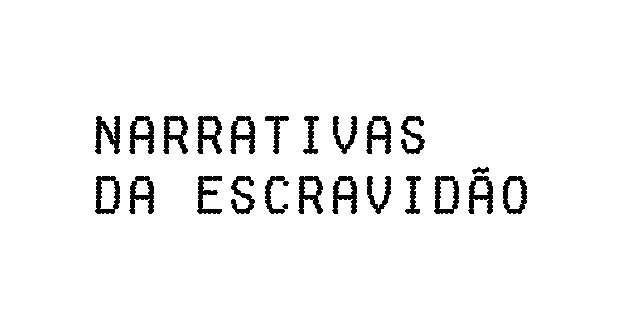
\includegraphics[width=.42\textwidth,keepaspectratio]{img/narrativas.eps}\par
%}{\large\textsc{narrativas da escravidão}}

%

%\begin{enumerate}
%\setlength{\topsep}{2pt}
%\setlength{\partopsep}{0pt}
%\setlength\parskip{4.2pt}
%\setlength\itemsep{-1.4mm}
%\item \textit{Incidentes da vida de uma escrava}, Harriet Jacobs
%\item \textit{Nascidos na escravidão: depoimentos norte-americanos}, \textsc{wpa}
%\item \textit{Narrativa de William W. Brown, escravo fugitivo}, William Wells Brown
%\end{enumerate}

%

\IfFileExists{img/ANARC.pdf}{%
  \vspace*{0mm}%
  \begin{enumerate}
    \setlength{\topsep}{0pt}\setlength{\partopsep}{0pt}\setlength{\itemsep}{0pt}\setlength{\parsep}{0pt}
    \item[] \noindent\hspace*{-1em}
\includegraphics[width=.42\textwidth,keepaspectratio]{img/ANARC.pdf}\par
  \end{enumerate}
}{\large\textsc{anarc}}



\begin{enumerate}
\setlength{\topsep}{2pt}
\setlength{\partopsep}{0pt}
\setlength\parskip{4.2pt}
\setlength\itemsep{-1.4mm}
\item \textit{Ação direta}, Voltairine de Cleyre
\item \textit{Anarquia pela educação}, Élisée Reclus
\item \textit{Entre camponeses}, Malatesta
\item \textit{Escritos revolucionários}, Malatesta
\item \textit{História da anarquia} (v.\,1), Max Nettlau
\item \textit{História da anarquia} (v.\,2), Max Nettlau
\item \textit{O indivíduo, a sociedade e o Estado, e outros ensaios}, Emma Goldman
\item \textit{O princípio anarquista e outros ensaios}, Kropotkin
\item \textit{O princípio do Estado e outros ensaios}, Bakunin
\item \textit{Os sovietes traídos pelos bolcheviques}, Rocker
\item \textit{Revolução e liberdade: cartas de 1845 a 1875}, Bakunin
\item \textit{Sobre anarquismo, sexo e casamento}, Emma Goldman
\end{enumerate}


%

%\IfFileExists{img/ecopolitica.eps}{%
%  \vspace*{0mm}\noindent
\includegraphics[width=.42\textwidth,keepaspectratio]{img/ecopolitica.eps}\par
%}{\large\textsc{ecopolítica}}

%

%\begin{enumerate}
%\setlength{\topsep}{2pt}
%\setlength{\partopsep}{0pt}
%\setlength\parskip{4.2pt}
%\setlength\itemsep{-1.4mm}
%\item \textit{Anarquistas na América do Sul}, E.\,Passetti, S.\,Gallo; A.\,Augusto  (org.)
%\item \textit{Ecopolítica}, E.\,Passetti; A.\,Augusto; B.\,Carneiro; S.\,Oliveira, T.\,Rodrigues  (org.)
%\item \textit{Pandemia e anarquia}, E.\,Passetti; J.\,da Mata; J.\,Ferreira  (org.)
%\end{enumerate}


\endgroup % fecha o grupo
\nopagecolor
\color{black}